\section*{Exercício 5}

Consideremos os referenciais \(\Sigma\) de repouso do túnel e \(\Sigma'\) de repouso do trem. Em \(\Sigma,\) como tanto o túnel quanto o trem são medidos com comprimento \(L\), portanto existe um instante em que as extremidades do túnel e do trem são coincidentes, denotados pelos eventos \(A\) e \(B\) no diagrama de espaço-tempo abaixo. Entretanto, o evento \(B\), em que a frente do trem coincide com a saída do túnel, só é simultâneo ao evento \(A\), em que a parte de trás do trem coincide com a entrada do túnel, no referencial \(\Sigma\): no referencial \(\Sigma'\), o evento \(B\) é simultâneo com o evento \(D\), onde a traseira do trem se encontra antes de entrar no túnel, e o evento \(A\) é simultâneo com o evento \(C\), onde a parte frontal do trem se encontra após a saída do túnel. Desse modo, os eventos simultâneos a \(A\) e \(B\) são compatíveis com a observação em \(\Sigma'\) de que o túnel é menor do que o trem, visto que neste referencial sempre que uma extremidade do trem é coincidente com uma extremidade do túnel, há uma porção do trem externa ao túnel. Concluímos portanto que ambas as observações são válidas, devido ao fato de que a simultaneidade não é absoluta.

\begin{figure}[H]
    \centering
    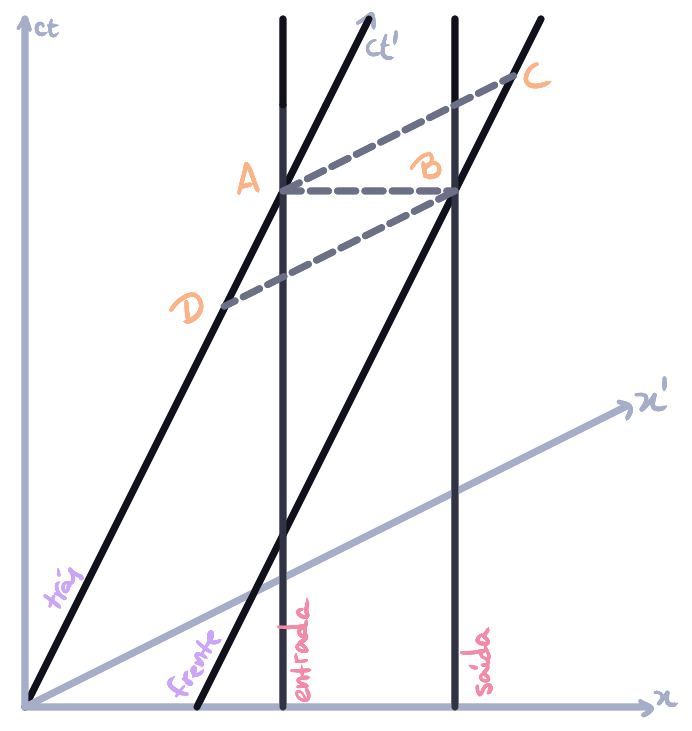
\includegraphics[width=0.5\textwidth]{tunel_trem.png}
    \caption{Diagrama de espaço-tempo}
\end{figure}

